% 连通性
% 连通性|连通空间|闭集|开集|拓扑空间|连通子集|同胚

\pentry{连续映射和同胚\upref{Topo1}}

\subsection{连通性的概念}
什么叫连通性?直观来说,在平面$\mathbb{R}^2$上画两个不相交也不相切的圆,那么这两个圆所包含的区域就是不连通的.不连通的各部分显然是可以被“孤立”出来的,也就是说,如果两圆不相交也不相切,就一定能各自找到一个开集,让这两个圆分别被一个开集包含,而这两个开集还互不相交.这就是定义连通性的方法.

我们把这两个圆包含的区域单独拿出来,构造一个子空间.在这个子空间中,两个圆各自有一个特点:它们既是开集也是闭集.如果将两个圆分别记为$C_1$和$C_2$,子空间记为$A=C_1\cup C_2$,包含它们的开集分别是$U_1\supseteq C_1$和$U_2\supseteq C_2$,且$U_1\cap U_2=\varnothing$,那么由子拓扑的定义,$C_1=C_1\cap U_1$是子空间的开集,同理$C_2$也是子空间的开集;然而在子空间中还有$C_1=A-C_2$,所以$C_1$还应该是一个闭集,同理$C_2$也是一个闭集.

\begin{figure}[ht]
\centering
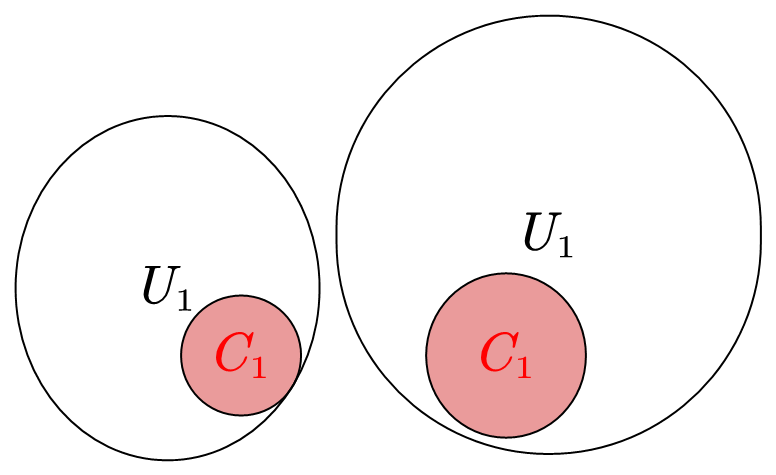
\includegraphics[width=6cm]{./figures/Topo3_1.png}
\caption{$C_1$,$C_2$,$U_1$和$U_2$的示意图} \label{Topo3_fig1}
\end{figure}

如果你选择的是一个连通的空间,比如说一个圆所包含的区域构造的子空间,那么这种“既开又闭”的情况是不会存在的.因此,我们可以根据既开又闭的性质来定义连通性.

\begin{definition}{孤立分支}
给定拓扑空间$X$和它的一个非空真子集$A$.如果$A$在$X$中既是开集也是闭集,那么称$A$是$X$的一个\textbf{孤立分支}.
\end{definition}

注意,定义孤立分支的时候特别强调了$A$是一个非空真子集,这样就把$\varnothing$和$X$本身排除在外了,因为按照定义,它们俩必须是既开又闭的.在上图中的$C_1$和$C_2$就是两个孤立分支.

有了孤立分支的概念,就能直接引入连通性的概念了:

\begin{definition}{连通性}
拓扑空间$X$是\textbf{连通(connected)}的,当且仅当$X$中没有孤立分支.
\end{definition}

连通性也可以用别的方式定义.

\begin{exercise}{连通性的等价定义}\label{Topo3_exe1}
给定拓扑空间$X$,证明“$X$是连通的”和以下命题等价:
\begin{itemize}
\item $X$不可以表示为两个非空不相交的开集的并;
\item $X$不可以表示为两个非空不相交的闭集的并;
\item 如果$B$是只有两个元素的离散拓扑,那么不存在$X$到$B$的满射.

\end{itemize}
\end{exercise}

对于任何拓扑空间,我们可以讨论这个空间本身是不是连通的,也可以研究各个子集构成的子空间是不是连通的.如果一个子集作为拓扑空间是连通的,我们就说这是一个\textbf{连通子集(connected subset)}

\begin{example}{$\sin{\frac{1}{x}}$}\label{Topo3_ex3}
在$(0,\infty)$上定义函数$\sin{\frac{1}{x}}$,取函数图像上的所有点的集合作为$\mathbb{R}^2$的子集:$S=\{(x, y)|x>0, y=\sin{\frac{1}{x}}\}$.取$S$的闭包$\bar{S}$,那么$S$和$\bar{S}$都是连通的.
\end{example}

\subsection{连通性的性质}

引入连通性的概念,一个关键的好处是它刻画了拓扑空间的一个基本性质.正如我们在同胚\upref{Topo1}中提过的,连通性是一个同胚不变性,也就是说,同胚的拓扑空间的连通性是完全一致的.这由以下定理保证:

\begin{theorem}{连通性的同胚不变性}\label{Topo3_the1}
设有拓扑空间$X$和$Y$,令$f:X\rightarrow Y$是一个连续映射,那么,对于$X$的任何连通子集$A$,$f(A)$也是$Y$的连通子集.
\end{theorem}

应用“开集的逆映射还是开集”可以很容易地证明这一定理.考虑到同胚映射在两个方向($X\rightarrow Y$和$Y\rightarrow X$)上都是连续映射,那么同胚映射把两个拓扑空间的连通子集彼此对应起来了.

在\autoref{Topo3_ex3}中我们知道$S$和$\bar{S}$都是连通的,这不是偶然的.

\begin{theorem}{闭包的连通性}\label{Topo3_the2}
给定拓扑空间$X$和它的一个连通子集$A$.如果$A\subseteq B\subseteq\bar{A}$,那么$B$也是连通的.特别地,$\bar{A}$是连通的.
\end{theorem}

由\textbf{集合的内部、外部和边界}词条中\autoref{Topo0_cor1}可知,\autoref{Topo3_the2}中定义的$B$就是$A$添上若干边界点生成的;如果把边界点全都添上了,那就是$\bar{A}$.